% vim: set filetype=tex

\section{\color{fancy}Chapter 5: Feature Indicator}

\begin{figure}[h]
  \centering
  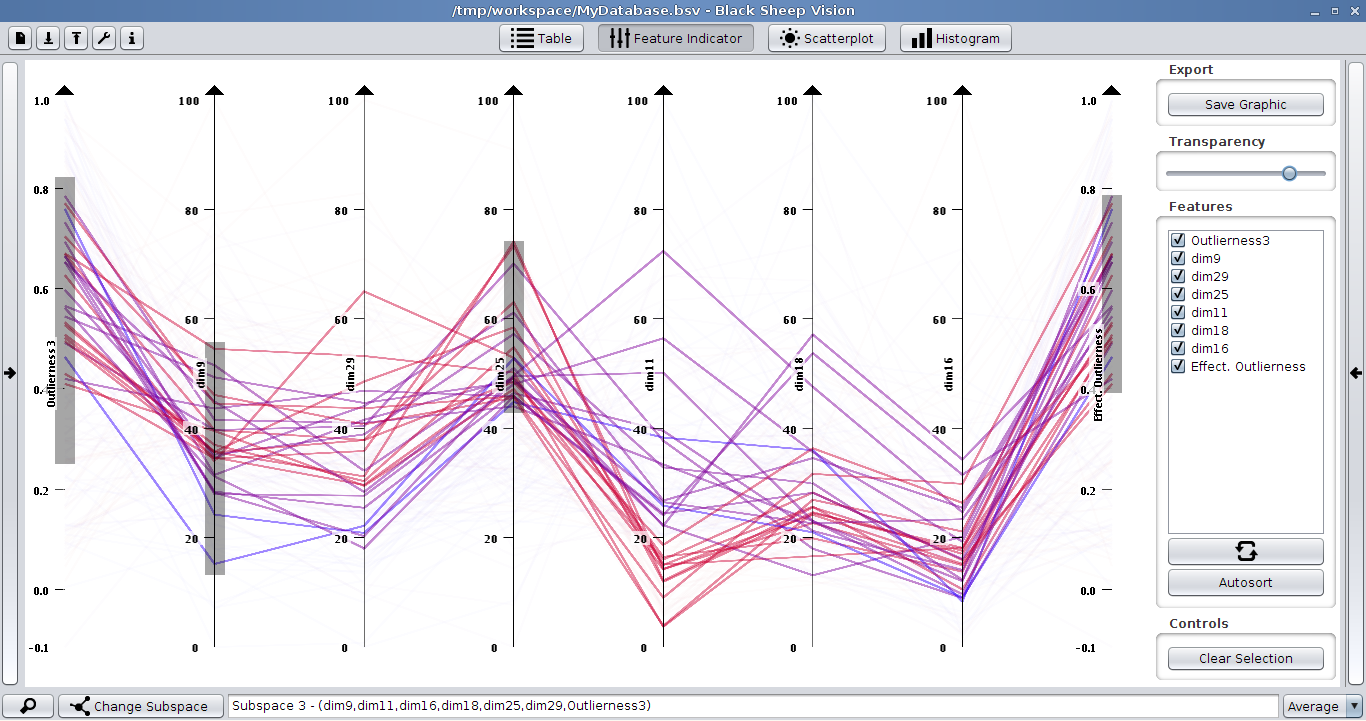
\includegraphics[width=16cm]{images/bsv/FeatureIndicator.png}
  \caption{Feature Indicator}
  \label{fig:featureindicator}
\end{figure}

\subsection{Functionality}
\begin{tabular}{p{0.2\linewidth}p{0.7\linewidth}}
  \color{fancy}Feature & \color{fancy}Usage \\ \hline
  Display & The Feature Indicator shows all currently available features side by side, with each value of an element connected by a line.  \\ \hline
  Control & On the right side you find various control mechanisms. You are able to adjust the transparency of the view, independent from each group's transparency, export the current view (e.g. as a \textbf{.svg}) or change the visibility of specific features. \\ \hline
  Rearrange &  You are able to rearrange the features by simple drag and drop gestures, within the list of features. Keep in mind to update the view, by clicking on the update button, below the list, after rearranging.\\ \hline
  Autosort &  By using the autosort functionality, the active features are automatically sorted, according to their correlation coefficient. This should give you good arrangement for a first overview, thus it is recommended to use, if your data consists of a large number of features (i.e. ten or more).  \\ \hline
  Select & You are able to select ranges of a specific feature by using your mouse to drag a bar at the feature axis. To discard all selections, you have to click the clear selection button, at the bottom of the control menu. \\ \hline
\end{tabular}

\subsection{Shortcuts}
\begin{center}
  \begin{spacing}{2.5}
  \begin{tabular}{c|l}
    \color{fancy}Shortcut & \color{fancy}Function\\
    \hline\hline
    \Ctrl + \keystroke{R} & Resets the selection.\\
  \end{tabular}
  \end{spacing}
\end{center}
